%% ID: simple_ladder_leaning
%% TITLE: Leaning ladder
%% TYPE: question
%% QUESTIONTYPE:  scq
%% CONCEPTS: forces, hooke, moments, vectors1, vectors2, trig
%% VIDEOS: 
%% LEVEL: 4
%% TOPIC: mechanics/statics
%% ORDER: 3

\begin{problem} [simple_ladder_leaning]
{\exposition{A uniform ladder of mass \vari{m} and length \vari{l} leans against a frictionless wall at an angle \vari{\theta} to the horizontal, with its bottom resting on a rough surface with a coefficient of friction \vari{\mu}.}\question{If \valuedef{\theta}{30^{\circ}}{}, what is the minimum value for \vari{\mu} so that the ladder does not slip?}

\begin{enumerate}

\item \choice[a]{\valuedef{\mu}{\frac{1}{2}}{}}
\item \choice[b]{\valuedef{\mu}{\frac{1}{\sqrt{3}}}{}}
\item \choice[c]{\valuedef{\mu}{\frac{1}{\sqrt{2}}}{}}
\item \choice[d]{\valuedef{\mu}{\frac{\sqrt{3}}{2}}{}}\correct
\item \choice[e]{\valuedef{\mu}{1}{}}

\end{enumerate}
}
{\textit{Created for the Rutherford School Physics Project by MC.}}
{\answer{The answer is d.} The only forces acting on the ladder in the vertical direction are the normal reaction of the floor on the ladder \vari{N_f} and its weight  \vari{mg}, so $N_f = mg$. Resolving horizontally, the frictional force between the floor and the ladder,  \vari{F_f}, balances out the normal reaction force of the wall on the ladder,  \vari{N_w}, so $N_w = F_f$

\begin{figure}[h]
\centering
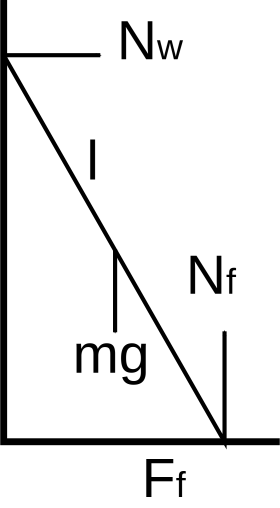
\includegraphics[width=0.3\textwidth]{../../../figures/statics_simple_ladder.svg}
\caption{} \label{fig:statics_simple_ladder}
\end{figure}

Taking moments around the top of the ladder: \begin{equation*} \frac{mgl}{2}\cos\theta = F_f l \sin\theta\end{equation*}
\begin{equation*} F_f = \frac{mg}{2\tan\theta}\end{equation*}. The maximum value of \vari{F_f} is \begin{equation*} F_f = \mu N_f = \mu mg\end{equation*}, and equating these to get the corresponding minimum value for \vari{\mu} gives \begin{equation*} \mu = \frac{1}{2\tan\theta}\end{equation*}. For \valuedef{\theta}{30^{\circ}}{}, this gives \begin{equation*} \mu = \frac{\dqrt{3}}{2}\end{equation*}.
}
\end{problem}